
\begin{table*}[t] 
 
 \begin{center}
 \begin{tabular} {| c | c | c c c | c c c |}
 \hline
 Competition & Year & TM Software & Open-Source & Maps & 1st Place & 2nd Place & 3rd Place\\
 \hline
 AIIDE & 2010 & Manual & Optional & Unannounced & Overmind & Krasi0 & Chronos \\
 \hline
 AIIDE & 2011 & AIIDE TM & Forced & Announced & Skynet & UAlbertaBot & Aiur \\
 \hline
 AIIDE & 2012 & AIIDE TM & Forced & Announced & Skynet & Aiur & UAlbertaBot\\
\hline
 AIIDE & 2013 & AIIDE TM & Forced & Announced & UAlbertaBot & Skynet & Aiur\\
\hline
 AIIDE & 2014 & AIIDE TM & Forced & Announced & IceBot & Ximp & LetaBot\\
\hline
 AIIDE & 2015 & AIIDE TM & Forced & Announced & tscmoo & ZZZKBot & Overkill\\
\hline
 AIIDE & 2016 & AIIDE TM & Forced & Announced & Iron & ZZZKBot & tscmoo\\
\hline
 AIIDE & 2017 & AIIDE TM & Forced & Announced & ZZZKBot & PurpleWave & Iron\\
\hline
 CIG & 2011 & Manual & Optional & Unannounced & Skynet & UAlbertaBot & Xelnaga\\
 \hline
 CIG & 2012 & AIIDE TM & Optional & Unannounced & Skynet & UAlbertaBot & Xelnaga\\
 \hline
 CIG & 2013 & Java-based TM & Optional & Unannounced & Skynet & UAlbertaBot & Aiur\\
 \hline
 CIG & 2014 & AIIDE TM & Forced & Unannounced & IceBot & Ximp & LetaBot\\
 \hline
 CIG & 2015 & AIIDE TM & Optional & Unannounced & ZZZKBot & tscmoo & Overkill\\
 \hline
 CIG & 2016 & AIIDE TM & Forced & Announced & tscmoo & Iron & LetaBot\\ 
 \hline
 CIG & 2017 & AIIDE TM & Forced & Announced & ZZZKBot & tscmoo & PurpleWave\\ 
 \hline   
 SSCAIT & 2011 & Custom & Optional & Announced & Roman Danielis & N/A & N/A\\
 \hline
 SSCAIT & 2012/13 & Custom & Optional & Announced & DementorBot & Marcin Bartnicki & UAlbertaBot\\
 \hline
 SSCAIT & 2013/14 & Custom & Optional & Announced & Ximp & WOPR & UAlbertaBot \\
 \hline
 SSCAIT & 2014/15 & AIIDE TM + Mod & Optional & Announced & LetaBot & WOPR & UAlbertaBot\\
 \hline
 SSCAIT & 2015/16 & AIIDE TM + Mod & Optional & Announced & LetaBot & Carsten Nielsen & UAlbertaBot \\
 \hline
 SSCAIT & 2016/17 & AIIDE TM + Mod & Optional & Announced & LetaBot & Wulibot & Zia Bot\\
 \hline
 SSCAIT & 2017/18 & AIIDE TM + Mod & Optional & Announced & Wulibot & LetaBot & Carsten Nielsen\\
 \hline
 \end{tabular}
 \end{center}  
 \caption{Tournament settings and top 3 finishers in the AIIDE, CIG, and SSCAIT (Student Division) competitions.}
 \label{tableTournaments}
\end{table*} 

\section{Current StarCraft Bots}\label{secBots}

Over the years, StarCraft AI competitions have motivated many individuals and groups to implement a variety of bots capable of playing complete StarCraft 1v1 games. Bots vary in complexity, and while many are rule-based, top-performing bots are now employing more sophisticated AI techniques such as real-time search/planning, pre-trained neural network controllers, and online learning during the competition games.

In this section, we provide an overview of a selection of bots and discuss some of the AI approaches they implement. We only mention those bots that are currently active in one of the competitions, have recently been updated, and employ some more complex AI techniques. 

\begin{itemize}
  \setlength\itemsep{1em}
  
%  \item {\em AIlien:} AIlien is a relatively new Zerg bot. Various kinds of its decisions rely on ``scoring'' systems. Other than that, it employs state machines -- especially for higher-level strategy and macro decisions.
  
  \item {\em CherryPi:} CherryPi is a TorchCraft \cite{synnaeve2016torchcraft} Zerg bot developed by Facebook AI Research team. 
  It is implemented as a collection of heterogenous modules that can be added, removed, or configured via the command line. This design allows individual modules to be easily replaced with learning-powered modules, or to do narrow experiments using only a subset of them. The modules communicate by exchanging two kinds of data elements via the blackboard architecture: Key-value pairs and so-called UPC objects (Unit, Position, Command), which have a generic enough meaning to be loosely interpreted by other modules. In general, a UPC represents a probability distribution of units, a probability distribution of positions and a single command. Build orders are represented as a set of prioritized requests pushed into a queue that fills in requirements and applies optimizations (like allocating resources for just-in-time construction). Fight-or-flight decisions are made by clustering units and running a combat simulation. CherryPi's combat simulation works similarly to SparCraft simulation package (see UAlbertaBot) with a naive ``attack-the-closest-target'' policy for enemy behavior. A threat-aware path-finding is used to find the least dangerous routes to a safety. The selection of high-level strategy across multiple games is based on UCB1 algorithm, selecting from a fixed list of strategies against each race. The bot uses TorchCraft to communicate with BWAPI over TCP, which allows it to run on a different host than StarCraft.
  
  \item {\em cpac:} A Zerg bot created by a 13-person team from China, cpac combines hard-coded rules with a multi-layer perceptron network for unit production. The network is trained on state-action pairs extracted from a large data set of BroodWar games \footnote{\url{http://www.starcraftai.com/wiki/StarCraft_Brood_War_Data_Mining}}. The core of cpac bot is based on the bots UAlbertaBot and Steamhammer (see below).
  
  \item {\em ForceBot:} ForceBot is a Zerg bot written in GOAL -- an agent-based programming language designed on top of BWAPI for programming cognitive agents.\footnote{\url{http://goalapl.atlassian.net/wiki/spaces/GOAL/}} Since the GOAL language is designed to implement multi-agent systems, all of ForceBot's units have their own corresponding agent with specific beliefs and goals. Each agent more or less follows a rule-based AI pattern.  
  
%  \item {\em Ian Nicholas DaCosta:} This Protoss bot uses genetic algorithms for targeting, and detecting enemy army threat levels. Supervised learning was applied for the detection of opponent's strategies and builds.
  
  \item {\em Iron:\footnote{\url{http://bwem.sourceforge.net/Iron.html}}} Iron bot won the 2016 AIIDE competition, and is a decentralized multi-agent system, with each unit controlled by a highly autonomous individual agent, able to switch between 25 behaviors. All its units share one simple aim: go to the main enemy base and destroy it. It often seems like a harasser bot, which is due to its units having mainly individual behavior. There are also so-called ``expert'' agents who autonomously recommend how resources should be spent and what units should be trained, based on heuristics. 
  
 % \item {\em KaonBot:} For resource and unit allocation based on prioritized needs, KaonBot applies a competing priority algorithm. According to the author, the bot will learn these priorities from experience in future releases.
  
  \item {\em KillAll:} The KillAll bot is based on Overkill bot by Sijia Xu and most of its functionality is rule-based. However, its production module uses Q-learning to select unit types to produce based on the current situation. 
    
  \item {\em Krasi0bot:} Krasi0bot has competed every year since 2010, and is still being actively developed. Even though it originally started as a rule-based bot, it currently makes some use of genetic algorithms, neural networks and potential fields. Krasi0bot plays the Terran race, and is known for its strong defensive capabilities, and wide variety of strategies implemented. As Krasi0bot is not open-source, not much is known of the techniques it uses. 
  \begin{figure*}[t]
  \begin{center}
  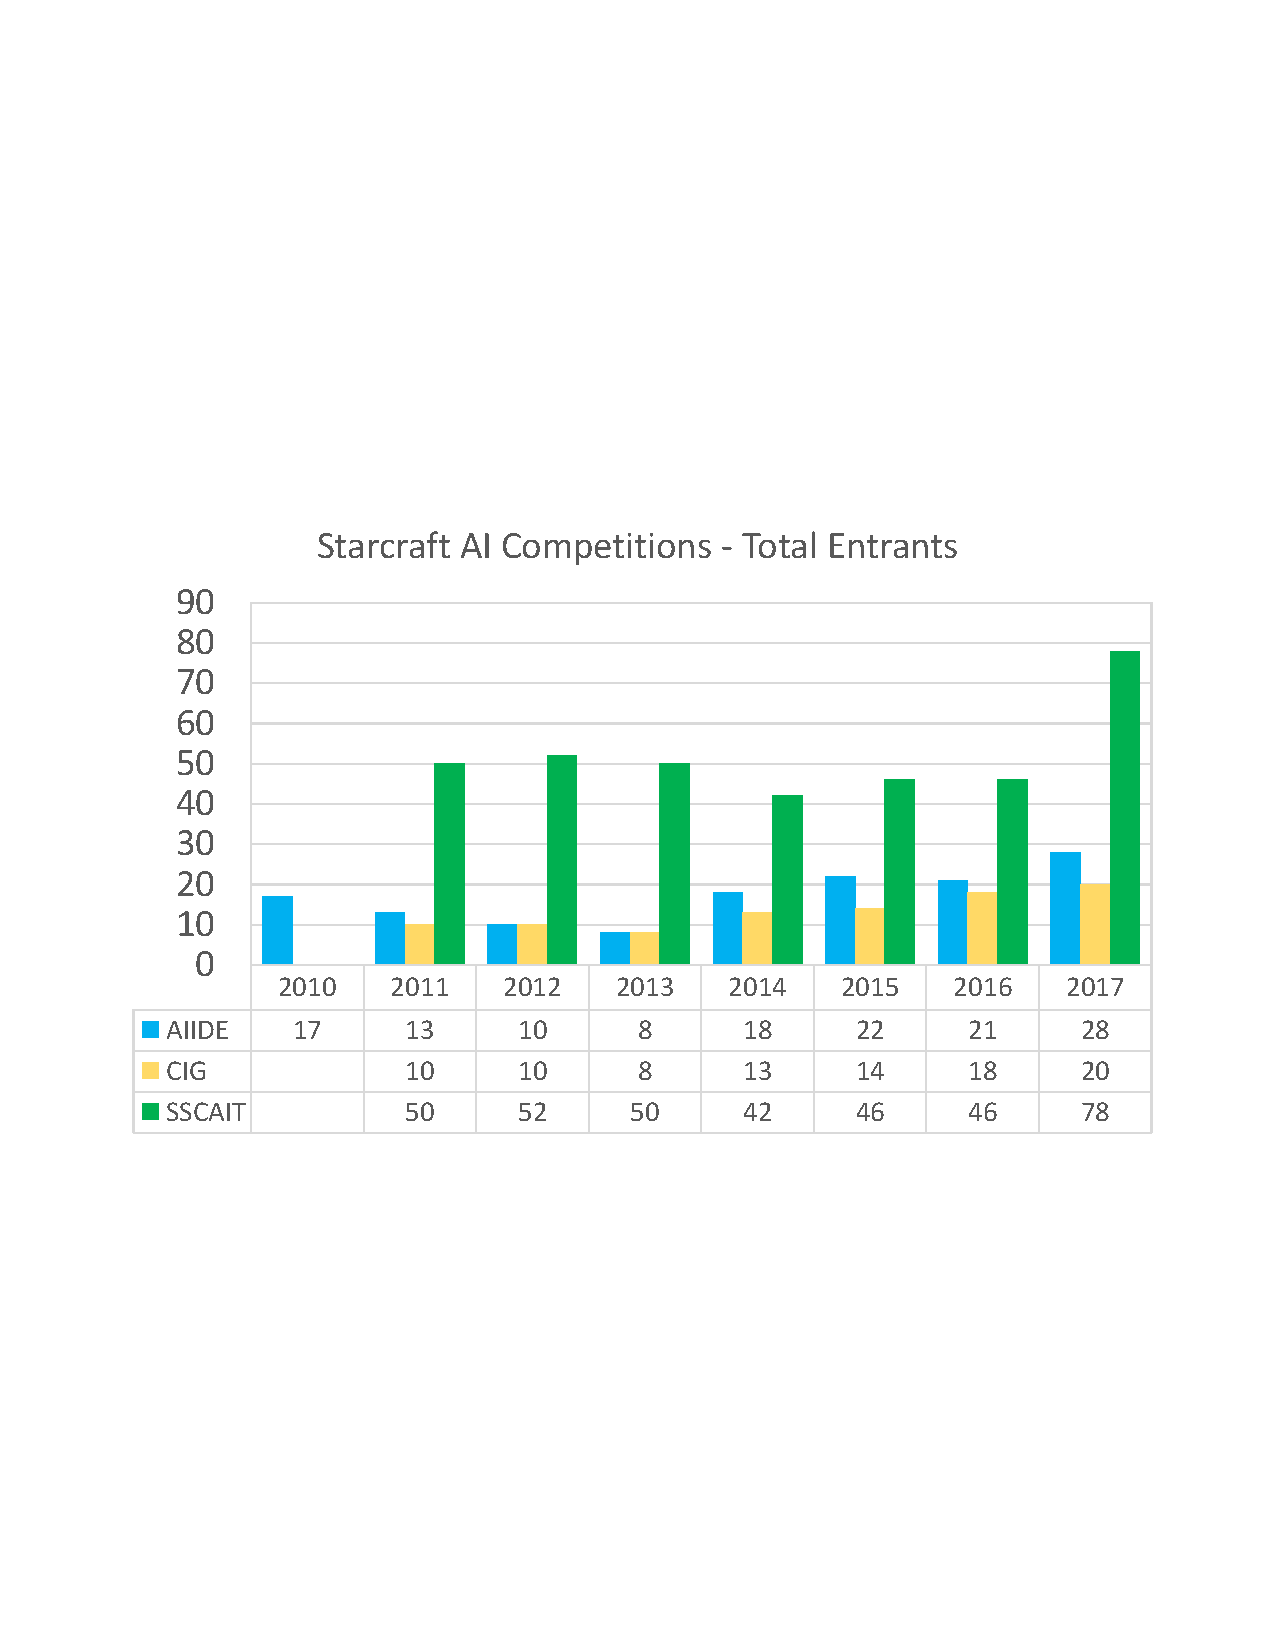
\includegraphics[width=9cm]{fig/Entrants}
	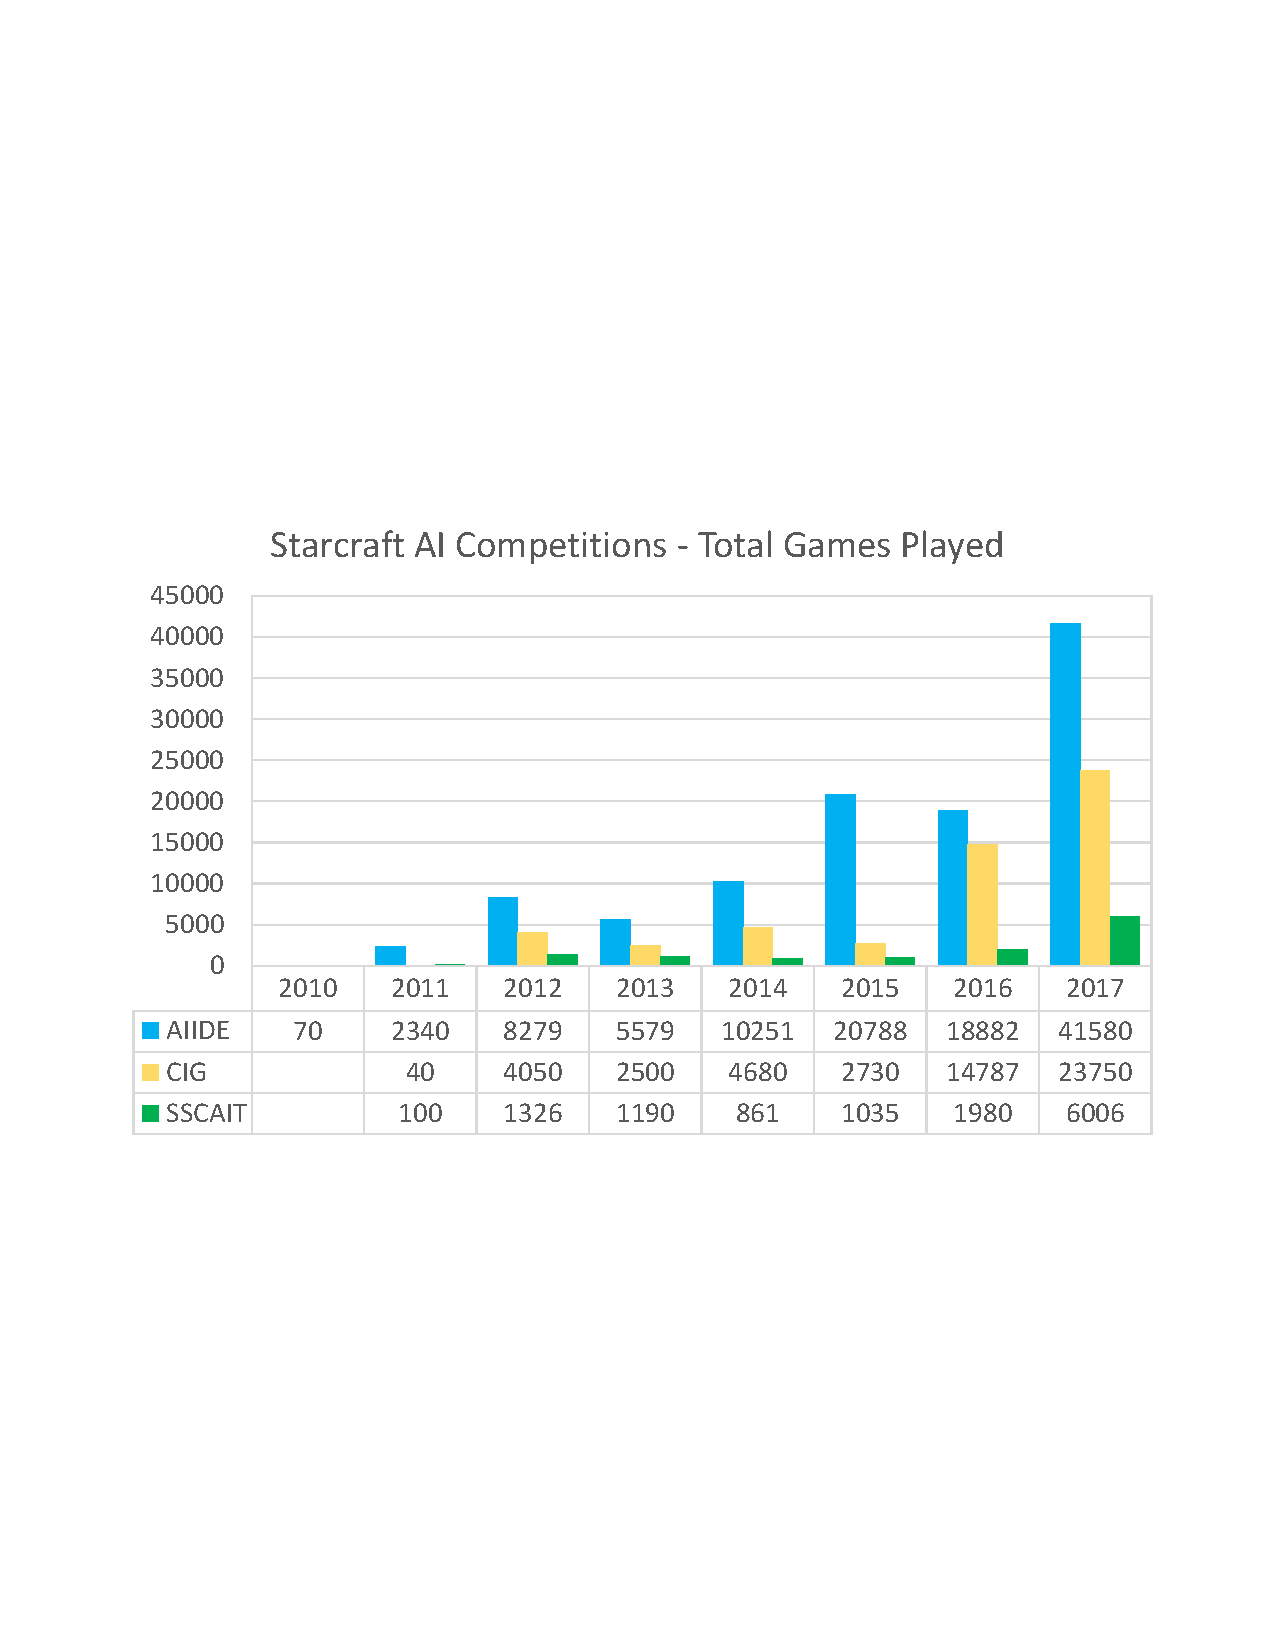
\includegraphics[width=9cm]{fig/GamesPlayed}
%  \vspace{-0.2cm}  
  \caption{Statistics for each of the 3 major annual StarCraft AI Competitions: AIIDE, CIG, and SSCAIT, since the first competition in 2010. Shown on the left is the number of total entrants for each competition, and on the right are the total number of games played in each competition.  }
  \label{fig:comps}
  \end{center}
  \vspace{-0.5cm}
\end{figure*}
  \item {\em LetaBot:\footnote{\url{https://github.com/MartinRooijackers/LetaBot}}} LetaBot won the 2014, 2015, and 2016 SSCAIT tournaments. It uses Monte Carlo Tree Search (MCTS) to plan the movement of groups of units around the map. A similar approach has previously been used by the author of Nova bot, Alberto Uriarte~\cite{uriarte2014high}. It employs cooperative pathfinding for resource gathering and text mining to extract build orders from Liquipedia articles.

  \item {\em McRave:} All the decisions of McRave bot are based on current enemy unit composition -- there are no hard-coded tech choices. The bot also builds an opponent model and uses it to select build orders. 

  \item {\em MegaBot:\footnote{\url{https://github.com/andertavares/MegaBot}}} For every game, MegaBot~\cite{tavares2016rock} chooses one of three approaches, each of which is implemented as a different bot (Skynet, Xelnaga or NUSBot). Algorithm selection is modeled as a multi-armed bandit. At the beginning of the game, an algorithm is selected using epsilon-greedy strategy. After the game, the reward is perceived (+1, 0, -1 for victory, draw and loss, respectively) and the value of the selected algorithm is updated via an incremental version of recency-weighted exponential average (Q-learning update rule).
  
%  \item {\em  Monica / Maria / Brenda:} Zerg, Protoss and Terran bots employing a game simulation inside the BEAM Erlang/OTP VM. It uses TorchCraft~\cite{synnaeve2016torchcraft}  -- a library for machine learning research on RTS games. The unit logic is written in Lua.
  
  \item {\em PurpleWave:\footnote{\url{https://github.com/dgant/PurpleWave}}} The decision making of PurpleWave bot is mainly based on hierarchical task networks. For micromanagement, it uses a hybrid squad/multi-agent approach and nearest neighbors clustering. The bot then simulates the outcomes of battles and suggests tactics for squads by min-maxing tactical approaches by each side (e.g. ``charge in'', ``run away'', or ``fight with workers''). In the end, each unit takes the tactical suggestion under advisement, but behaves independently. The units choose between approximately two dozen simple, reusable stateless behaviors. The bot heuristics include using potential fields for unit movement. Strategies are chosen based on results of previous games, race, map, and number of starting positions. It has a graph of strategy selections, like opening build orders paired with mid game transitions and late-game compositions.
  	
  \item {\em StarcraftGP:} StarcraftGP is the first StarCraft meta-bot -- a program that autonomously creates a program that autonomously plays StarCraft~\cite{garcia2015towards}. Currently, StarcraftGP v0.1 is using (Linear) Genetic Programming and it is able to directly write C++ code. Its first creations: Salsa and Tequila, have been the first bots not directly written by a human to participate in international competitions.

  \item {\em Steamhammer:\footnote{\url{http://satirist.org/ai/starcraft/steamhammer/}}} Zerg bot Steamhammer, developed by Jay Scott, and its random-race version Randomhammer both employ sophisticated combat simulation with alpha-beta search and portfolio search to predict the outcome of battles. The bots also use hierarchical reactive control for the units. For Protoss and Terran production, Randomhammer uses branch-and-bound search, while Zerg is currently rule-based.

  \item {\em tscmoo:\footnote{\url{https://github.com/tscmoo}}} tscmoo won the 2015 AIIDE and 2016 CIG competitions. The bot uses no external libraries: it has its own combat simulation code to predict the outcome of battles, it does not use BWTA\footnote{\url{http://bitbucket.org/auriarte/bwta2}} to analyze the terrain and it even has its own threat-aware path-finding for individual units. The bot is one of the most strategically diverse, and selects among its many strategies based on their success in previous games. Recent versions of the bot experimented with recurrent neural networks for high-level strategy and build order decisions.

  \item {\em UAlbertaBot:\footnote{\url{https://github.com/davechurchill/ualbertabot}}} UAlbertaBot has competed in every major StarCraft AI Competition since 2010, and won the 2013 AIIDE competition. UAlbertaBot uses a dynamic heuristic-search based Build-Order Search System (BOSS) to plan all its build-orders in real time, as well as a StarCraft combat simulation system called SparCraft for estimating the outcome of in-game battles. The bot uses the results of previous games against specific opponents to choose a strategy to implement at the beginning of each game, with each strategy being defined in an external JSON configuration file. Its development has focused on its ease of use and modification, and as such has become the basis of more than 10 other bots in current competitions, including LetaBot, Overkill, and Steamhammer. In 2017 UAlbertaBot became CommandCenter\footnote{\url{https://github.com/davechurchill/commandcenter/}}, the first bot capable of playing both BroodWar and StarCraft 2.
  
%  \item {\em V\'{a}clav Bayer:} Q-learning / Reinforcement Learning and Markov Decision Processes are used by this bot -- mainly to select a build order with respect to opponent's strategy.
  
  \item {\em ZZZKbot:\footnote{\url{https://github.com/chriscoxe/ZZZKBot}}} ZZZKBot, a Zerg bot developed by Chris Coxe, was the winner of the 2017 AIIDE and CIG competitions. Its overall strategy implements 4 simple 1-base rush strategies: 4-pool, Speedlings, Hydralisks, and Mutalisks. If the initial rush does not end the game, the bot switches to either Mutalisks or Guardians for the late game, while researching upgrades for all its units. The bot records win/loss information for each opponent, and uses this information to pick the best combination of strategy parameters for future games in a rule-based manner. The majority of the bots rules for unit control and micromanagement are simple rule-based behaviors based on expert knowledge prioritization.

\end{itemize}

%\subsection{AI Strengths and Weaknesses}

We can observe over the past few years that StarCraft AI bots are indeed getting stronger overall. In the AIIDE and CIG competitions, several bots from previous years are intentionally left in the next year to serve as a benchmark for progress, and we see each time that these benchmark bots do worse over time. Also, expert players and enthusiasts observe replays and note how they feel bots have gotten better or worse over time. Most notably, many of these expert players feel that the bots have been gradually adapting a more 'standard' playing style than earlier bots, who traditionally did one strategy such as a rush, but not much else. More modern bots have developed mid and even late game tactics that were not seen in earlier rushing bots. Overall, bots seem to be getting better at army composition, build-order selection, building placement, and overall game strategy. 

While the strongest bots currently play at an amateur human level, expert players have noted that they still appear to be weak in a few key areas. Most importantly, bots still seem quite weak at adapting their strategies dynamically during a match in response to information gained about their opponent. The majority of bots employ a playbook of several strategies that they choose from at the start of a match and follow through to the end of the game, with only a few bots attempting to dramatically change things if the opponent does something unexpected. This means that bots are still quite vulnerable to human players who are more easily able to change strategies and tactics as a game goes on. Current bots also seem quite vulnerable to the human ability to quickly identify bot patterns and behavior, and exploit this quickly during a match. For example, one human player during a human vs.\ machine match noted that one bot unit would chase his Zergling when it got close to the bots' units, and proceeded to run the Zergling next to the bot army, and then lead the bot on a wild goose chase throughout the entire map. The entire time, the bot may have been reasoning that its army could win the fight against the single Zergling unit, while not realizing that the human was just buying time until its army was ready for the final attack. This also illustrates one of the biggest challenges in all of artificial intelligence: understanding the long term effects of actions which have delayed rewards. An expert human is able to quickly understand that they are being exploited in such a way, and that it will have negative effects down the road, and is able to stop the behavior. This long-term vision that is so intuitive to humans remains a problem for current RTS AI.



